\documentclass{article}

\usepackage[final]{style}
\usepackage[utf8]{inputenc} % allow utf-8 input
\usepackage[T1]{fontenc}    % use 8-bit T1 fonts
\usepackage{hyperref}       % hyperlinks
\usepackage{url}            % simple URL typesetting
\usepackage{booktabs}       % professional-quality tables
\usepackage{amsfonts}       % blackboard math symbols
\usepackage{nicefrac}       % compact symbols for 1/2, etc.
\usepackage{microtype}      % microtypography
\usepackage{verbatim}
\usepackage{graphicx}       % for figures

\title{Lecture \#6: Reconstrução 3D: Formas a partir de sombra, estéreo, textura e foco. Detecção de profundidade usando sensores ativos. Representação de superfícies e reconstrução baseada em modelos.}

\author{
  Felipe Torres Minorelli, Kevin Perondi Regis, Renan Viana Hoshi \\
  Department of Computer Science\\
  Federal University of Technology - Paran\'{a} / UTFPR\\
  Campo Mour\~{a}o, Paran\'{a}, Brazil \\
  \texttt{\{felipeminorelli,kevinperondi,renanvianah\}@gmail.com} \\
}

\begin{document}

\maketitle


\section{Introdução}

O presente trabalho tem como objetivo realizar uma abordagem sobre os tópicos necessários para realizar uma reconstrução 3D. As informações foram retiradas do capítulo 12 do livro \textit{Computer Vision: Algorithms and Applications} de  Richard Szeliski \cite{Szeliski:2010}. Os tópicos discutidos serão Formas a partir de sombra, estéreo, textura e foco. Detecção de profundidade usando sensores ativos. Representação de superfícies e reconstrução baseada em modelos.

\section{Formas a partir de sombra, estéreo, textura e foco}

Neste capítulo realizaremos o estudo de como formas podem ser inferidas a partir do sombreamento, textura e foco. Assim como estas 3 instâncias podem ser utilizadas para a reconstrução da geometria de um objeto 3D.

\subsection{Formas a partir de sombra}

Ao se observar um objeto sombreado, podemos distinguir sua forma apenas com a variação de sombreamento. Tal fenômeno ocorre pois a superfície normal do objeto muda ao longo de seu exterior, desta forma temos uma variação do brilho já que o mesmo é decorrente entre a variação da orientação da superfície e o ângulo da iluminação incidente. Podemos observar estas mudanças na Figura~\ref{fig:sombra}.

\begin{figure}[!htb]
    \centering
    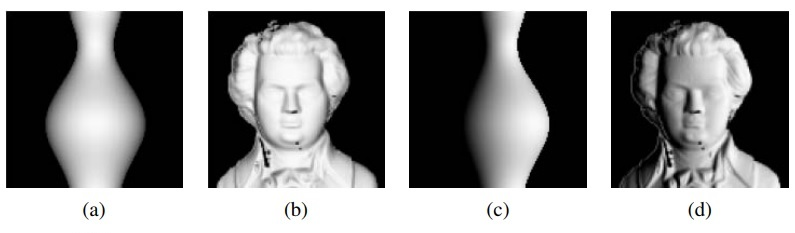
\includegraphics[width=0.90\textwidth]{imagem1.jpg}
    \caption{Forma sintética a partir de sombreamento (Zhang, Tsai, Cryer et al. 1999)}
    \label{fig:sombra}
\end{figure}

A recuperação da forma de uma superfície a partir desta variação é conhecida como \textit{shape from shading}, é um problema recorrente em visão computacional.
A maioria dos algoritmos de sombreamento assumem que o coeficiente de reflexão seja uniforme, e as direções da fonte de luz sejam conhecidas ou passiveis de alterações pelo uso de um objeto de referencia. A partir das suposições de observador e fontes de luz distantes, a variação de intensidade (equação de irradiância, Figura \ref{eq:irrad}) é baseada na orientação da superfície, onde (p,q) = (zx,zy) são as derivadas do mapa de profundidade e R(p,q) é o chamado mapa de reflectância.

\begin{figure}[!htb]
    \centering
    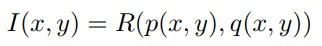
\includegraphics[width=0.60\textwidth]{equacao1.jpg}
    \caption{Equação de irradiância}
    \label{eq:irrad}
\end{figure}

Por exemplo uma superfície difusa, tem um mapa de reflectância calculado através do produto entre um ponto não negativo e a superfície normal e a direção da fonte de luz, Figura \ref{eq:mapareflec}, onde \textit{p} é é o fator de reflectância da superfície.

\begin{figure}[!htb]
    \centering
    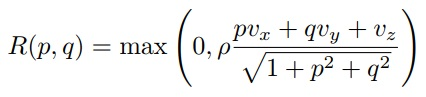
\includegraphics[width=0.60\textwidth]{equacao2.jpg}
    \caption{Equação do mapa de reflectância}
    \label{eq:mapareflec}
\end{figure}

Teoricamente as equações \ref{eq:irrad} e \ref{eq:mapareflec} podem ser utilizadas para se estimar (p,q), porém,  a não ser que outras restrições sejam adicionadas, ainda temos mais pares desconhecidos (p,q) do que intensidades calculadas (I). Uma das restrições mais utilizadas é a restrição de suavidade, Figura~\ref{eq:suavidade}. A outra é a restrição de integrabilidade, Figura~\ref{eq:integrabilidade}, onde para uma mapa de profundidade válido temos \textit{z(x,y)} com \textit{(p,q) = (zx,zy)}, portanto \textit{py = zxy = zyx = qx}.

\begin{figure}[!htb]
    \centering
    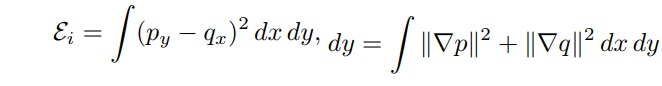
\includegraphics[width=0.60\textwidth]{equacao3.jpg}
    \caption{Restrição de suavidade}
    \label{eq:suavidade}
\end{figure}

\begin{figure}[!htb]
    \centering
    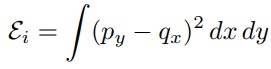
\includegraphics[width=0.60\textwidth]{equacao4.jpg}
    \caption{Restrição de integrabilidade}
    \label{eq:integrabilidade}
\end{figure}

Em vez de primeiro recuperar os campos de orientação \textit{(p, q)} e integrá-los para obter um
superfície, também é possível minimizar diretamente a discrepância na equação de formação de imagem
\ref{eq:irrad} ao encontrar o mapa de profundidade ideal \textit{z (x, y)}. Infelizmente, a forma
a partir do sombreamento é suscetível aos mínimos locais no espaço de busca, e como outros
problemas que envolvem a estimativa simultânea de muitas variáveis, também podem sofrer uma lenta convergência. Para diminuir este problema podemos nos utilizar de técnicas como a de multi-resolução (Szeliski 1991a) para acelerar a convergência, e as técnicas de otimização mais sofisticadas (Dupuis and Oliensis 1994), para a evitar mínimos locais.

Na prática, superfícies diferentes de modelos de gesso raramente possuem um coeficiente de reflectância uniforme. Portanto a reconstrução de forma a partir de sombreamento precisa ser combinado com alguma outra técnica ou estendido de alguma maneira para ter alguma utilidade. Uma maneira de fazer isso é a combinação com a correspondência estéreo (Fua e Leclerc 1995) ou textura conhecida (padrões de superfície) (White e Forsyth 2006), técnicas abordadas nas próximas seções. O estéreo e as componentes de textura fornecem informações em regiões texturizadas, enquanto a forma a partir de sombreamento ajuda preencha as informações em regiões uniformemente coloridas e também fornece informações mais detalhadas sobre a forma da superfície.

\subsection{Formas a partir do estéreo fotométrico}


Outra maneira de tornar a forma a partir do sombreamento mais confiável é utilização de várias
fontes de luz, que podem ser ativadas e desativadas seletivamente. Essa técnica é chamada de estéreo fotométrico. Uma vez que as fontes de luz desempenham um papel análogo às câmeras localizadas em diferentes locais, para cada fonte de luz, temos um mapa de refletância, \textit{R1 (p, q)}, \textit{R2 (p, q)}, etc, assim como as intensidades correspondentes \textit{I1}, \textit{I2}, etc. Em um pixel, podemos, em princípio, recuperar um coeficiente de reflectância desconhecido \textit{p} e uma orientação de superfície estimada \textit{(p, q)}. Para superfícies difusas (equação \ref{eq:mapareflec}), se parametrizarmos a orientação local por  \textit{nˆ}, obtemos (por pixeis não-sombreados) um conjunto de equações lineares da seguinte forma:

\begin{figure}[!htb]
    \centering
    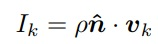
\includegraphics[width=0.3\textwidth]{equacao5.jpg}
    \label{eq:estereo}
\end{figure}

A partir do qual podemos recuperar \textit{pnˆ} usando mínimos quadrados lineares. Essas equações estão bem condicionadas desde que os vetores (três ou mais) \textit{vk} sejam linearmente independentes, isto é, não sejam
ao longo do mesmo azimute (direção oposta do observador). Uma vez que os normais ou gradientes da superfície tenham sido recuperados em cada pixel, eles podem ser integrado em um mapa de profundidade usando uma variante de ajuste de superfície regularizado. 

Quando as superfícies são especulares, podem ser necessárias mais de três direções de luz. De fato,
a equação de irradiância dada na Figura~\ref{eq:irrad} não requer apenas que as fontes de luz e a câmera sejam
distante da superfície, mas também negligencia as inter-reflexões, que podem ser uma fonte significativa
do sombreamento observado nas superfícies dos objetos, por exemplo, o escurecimento visto dentro das estruturas côncavas como ranhuras e fendas.

\subsection{Formas a partir da textura}

A variação no escorço observado em texturas regulares também pode fornecer informações úteis sobre a orientação da superfície local. Na Figura\ref{fig:textura} temos um exemplo desse padrão, ao longo
com as orientações de superfície locais estimadas. Algoritmos de formas a partir de textura requerem um número
etapas de processamento, incluindo a extração de padrões repetidos ou a medição de frequências para calcular deformações afins locais, e um estágio subsequente para inferir orientação de superfície.

\begin{figure}[!htb]
    \centering
    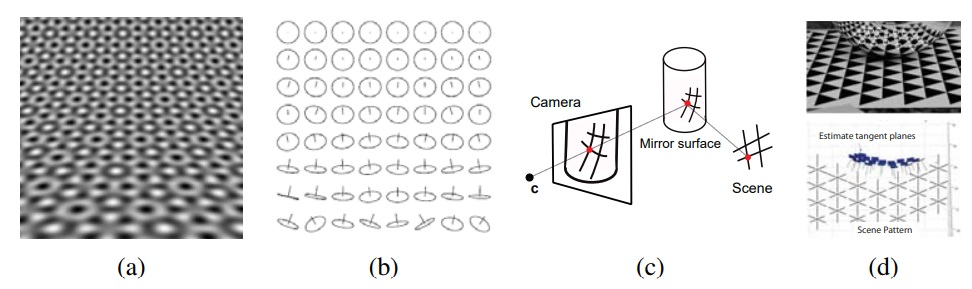
\includegraphics[width=0.9\textwidth]{imagem2.jpg}
    \caption{Forma sintética a partir da textura (Garding 1992)}
    \label{fig:textura}
\end{figure}


Quando o padrão original é regular, é possível ajustar um padrão regular, mas ligeiramente deformado, e usar essa grade para uma variedade de tarefas de substituição ou análise de imagens. Este processo torna-se ainda
mais fácil se padrões de tecido texturizado especialmente impressos forem usados. As deformações induzidas em um padrão regular, quando vistas na reflexão de um espelho curvo, como mostrado na Figura~\ref{fig:textura}, podem ser utilizadas para a recuperação da forma da superfície. Também é possível inferir informações de formas locais a partir do fluxo especular, ou seja, o movimento de especularidades quando visto de uma câmera em movimento.

\subsection{Formas a partir do foco}


Uma boa dica sobre a profundidade de um objeto é a quantidade de desfoque, que aumenta à medida que a superfície do objeto se afasta da distância de focagem da câmera. Movendo-se a superfície de um objeto para longe do plano de foco, aumentamos assim o círculo de confusão, quando calculado a partir de uma fórmula,podemos estabelecer esta característica facilmente.

Várias técnicas foram desenvolvidas para estimar a profundidade a partir da quantidade de desfocagem (profundidade de desfocagem) (Pentland 1987; Nayar and Nakagawa 1994; Nayar, Watanabe,
and Noguchi 1996; Watanabe and Nayar 1998; Chaudhuri and Rajagopalan 1999; Favaro
and Soatto 2006). Mas para que estas técnicas sejam efetivas é necessário levar em conta os seguintes problemas: 

\begin{enumerate}
    \item A quantidade de desfoque aumenta em ambas as direções à medida que você se afasta do plano de foco. Portanto, é necessário usar duas ou mais imagens capturadas com diferentes configurações de distância de foco, ou realizar a transformação das profundidades do objeto e analisar o ponto de nitidez máxima.
    \item A ampliação do objeto pode variar conforme a distância do foco é alterada ou o objeto é movido. Isso pode ser modelado explicitamente (tornando a correspondência mais difícil) ou a partir do uso da óptica telecêntrica, que aproxima uma câmera ortográfica e requer uma abertura na frente da lente.
    \item A quantidade de desfocagem deve ser estimada de maneira confiável. Uma abordagem simples é calcular a média quadrada do gradiente em uma região, mas tal abordagem pode sofrer de vários problemas, incluindo o problema de ampliação da imagem mencionado acima. Uma solução melhor é utilização de filtros racionais.

\end{enumerate}




\section{Detecção de profundidade usando sensores ativos}

Iluminar ativamente uma cena, seja para estimar as normais usando estéreo fotométrico ou para adicionar textura artificial para desfocar a forma, pode melhorar muito o desempenho dos sistemas de visão. Esse tipo de iluminação ativa tem sido usado desde os primeiros dias da visão de máquina para construir sensores altamente confiáveis para estimar imagens de profundidade 3D usando uma variedade de técnicas de detecção de alcance (Besl 1989; Curless 1999; Hebert 2000).

Um dos sensores de iluminação ativa mais populares é um sensor de laser ou faixa de luz, que varre um plano de luz através da cena ou objeto, observando-o de um ponto de vista desfocado (Rioux e Bird 1993; Curless e Levoy). 1995). Quando a listra cai sobre o objeto, ele deforma sua forma de acordo com a forma da superfície que está iluminando. É então uma simples questão de usar a triangulação óptica para estimar as localizações 3D de todos os pontos vistos em uma faixa específica. Em mais detalhes, o conhecimento da equação do plano 3D da faixa de luz nos permite inferir a localização 3D correspondente a cada pixel iluminado. A precisão das técnicas de \textit{striping} de luz podem ser melhoradas encontrando o pico temporal exato na iluminação de cada pixel (Curless e Levoy, 1995). A precisão final de um escaneamento pode ser determinada usando técnicas de modulação de borda inclinada, isto é, criando imagens de vincos nítidos em um objeto de calibração (Goesele, Fuchs e Seidel 2003).

\begin{figure}[!htb]
    \centering
    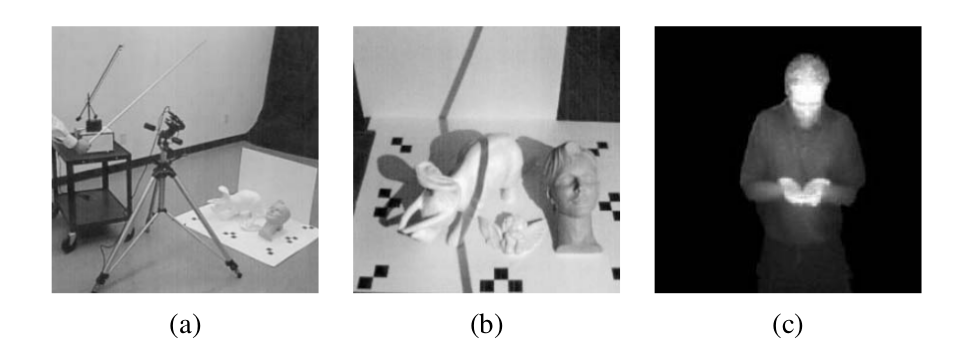
\includegraphics[width=1.0\textwidth]{escaneamentoDeFormas.png}
    \caption{Escaneamento de formas usando sombras projetadas (Bouguet e Perona 1999) ACM: (a) configuração da câmera com uma fonte de luz pontual (uma lâmpada de mesa sem seu refletor), um bastão manual projetando uma sombra e (b) os objetos sendo digitalizados na frente de dois fundos planares. (c) Mapa de profundidade em tempo real usando um sistema de iluminação pulsada (Iddan e Yahav 2001) c 2001 SPIE.}
    \label{fig:escaneamentoDeFormas}
\end{figure}

Uma variante interessante na identificação de faixas claras é apresentada por Bouguet e Perona (1999). Em vez de projetar uma faixa clara, eles simplesmente acenam com um bastão projetando uma sombra sobre uma cena ou objeto iluminado por uma fonte de luz pontual, como uma lâmpada ou o sol (Figura \ref{fig:escaneamentoDeFormas}a). Como a sombra cai em dois planos de fundo cuja orientação em relação à câmera é conhecida (ou inferida durante a pré-calibração), a equação plana para cada faixa pode ser inferida das duas linhas projetadas, cujas equações 3D são conhecidas (Figura \ref{fig:escaneamentoDeFormas}b) . A deformação da sombra ao cruzar o objeto que está sendo digitalizado revela sua forma 3D. Essa técnica também pode ser usada para estimar a geometria 3D de uma cena de fundo e como sua aparência varia à medida que ela se move na sombra, a fim de lançar novas sombras na cena (Chuang, Goldman, Curless et al. 2003).

O tempo que leva para digitalizar um objeto usando uma técnica de faixa de luz é proporcional ao número de planos de profundidade usados, que geralmente é comparável ao número de pixels em uma imagem. Um escaneamento mais rápido pode ser construído ligando e desligando diferentes pixels de projetor de uma maneira estruturada, por exemplo, usando um código binário ou Gray (Besl 1989). Por exemplo, vamos supor que o projetor LCD que estamos usando tenha 1024 colunas de pixels. Tomando o código binário de 10 bits correspondente ao endereço de cada coluna (0 ... 1023), projetamos o primeiro bit, depois o segundo, etc. Depois de 10 projeções, cada pixel da câmera sabe qual das 1024 colunas de luz do projetor está vendo. Uma abordagem semelhante também pode ser usada para estimar as propriedades de refração de um objeto colocando um monitor atrás do objeto (Zongker, Werner, Curless et al. 1999; Chuang, Zongker, Hindorff et al. 2000). Escaneamentos mais rápidos podem também ser construídos com um único feixe de laser, isto é, um escaneamento de triangulação óptica de pontos voadores em tempo real (Rioux, Bechthold, Taylor et al. 1987).

Se for necessária uma digitalização ainda mais rápida podemos projetar um único padrão texturizado na cena. Proesmans, Van Gool e Defoort (1998) descrevem um sistema no qual uma grade quadriculada é projetada em um objeto (por exemplo, a face de uma pessoa) e a deformação da grade é usada para inferir a forma 3D. Infelizmente, tal técnica só funciona se a superfície for contínua o suficiente para ligar todos os pontos da grade.

Um sistema consideravelmente melhor pode ser construído usando iluminação customizada de alta velocidade e \textit{hardware} de detecção. Iddan e Yahav (2001) descrevem a construção de sua câmera de detecção de profundidade com taxa de vídeo 3DV Zcam, que projeta um plano de luz pulsado sobre a cena e então integra a luz de retorno por um curto intervalo, obtendo essencialmente medidas de tempo de vôo para a distância dos pixels individuais na cena.

Em vez de usar uma única câmera, também é possível construir um sensor de faixa de iluminação ativa usando configurações de imagem estéreo. A maneira mais simples de fazer isso é apenas projetar padrões aleatórios de faixas na cena para criar uma textura sintética, que ajuda a combinar superfícies sem textura (Kang, Webb, Zitnick et al. 1995). A projeção de uma série conhecida de faixas, assim como na identificação de intervalo de uma única câmera codificada, torna a correspondência entre os pixels não ambígua e permite a recuperação de estimativas de profundidade em pixels vistos apenas em uma única câmera (Scharstein e Szeliski 2003). Esta técnica tem sido usada para produzir um grande número de pares estéreos multi-imagem registrados altamente precisos e mapas de profundidade com a finalidade de avaliar algoritmos de correspondência estéreo (Scharstein e Szeliski 2002; Hirschmüller e Scharstein 2009) e os antecedentes e parâmetros do mapa de profundidade de aprendizagem (Scharstein e Pal 2007).

\begin{figure}[!htb]
    \centering
    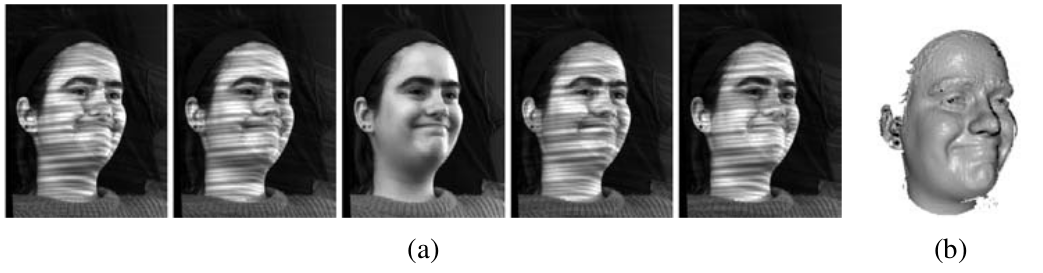
\includegraphics[width=0.8\textwidth]{mapaProfundidade.png}
    \caption{Captura de rosto 3D densa em tempo real usando estéreo no espaço tempo (Zhang, Snavely, Curless et al. 2004) ACM: (a) conjunto de cinco quadros de vídeo consecutivos de uma das duas câmeras estéreo (a cada quinto quadro é livre de padrões de faixa) para extrair textura); (b) resultante modelo de superfície 3D de alta qualidade (mapa de profundidade visualizado como uma renderização sombreada).}
    \label{fig:mapaProfundidade}
\end{figure}

Embora a projeção de vários padrões geralmente exija que a cena ou o objeto permaneçam imóveis, o processamento adicional pode permitir a produção de mapas de profundidade em tempo real para cenas dinâmicas. A ideia básica (Davis, Ramamoorthi e Rusinkiewicz 2003; Zhang, Curless e Seitz 2003) é assumir que a profundidade é quase constante dentro de uma janela espaço-temporal 3D em torno de cada pixel e usar a janela 3D para correspondência e reconstrução. Dependendo da forma da superfície e do movimento, essa suposição pode ser propensa a erros, como mostrado em (Davis, Nahab, Ramamoorthi et al. 2005). Para modelar formas com maior precisão, Zhang, Curless e Seitz (2003) modelam a variação de disparidade linear dentro da janela espaço-tempo e mostram que melhores resultados podem ser obtidos otimizando globalmente as estimativas de gradientes de disparidade sobre volumes de vídeo (Zhang, Snavely, Curless et al., 2004). A Figura \ref{fig:mapaProfundidade} mostra os resultados da aplicação desse sistema no rosto de uma pessoa; o modelo de superfície 3D com taxa de quadros pode ser usado para manipulação de gráficos e computação gráfica baseada em modelo.

\subsection{Fusão de dados de faixa (\textit{Range data merging})}
\label{subSec:rangeDataMerging}

Embora as imagens de alcance individual possam ser úteis para aplicações como z-keying em tempo real ou captura de movimento facial, elas são frequentemente usadas como blocos de construção para modelagem de objetos 3D mais completa. Em tais aplicações, os próximos dois passos no processamento são o registro (alinhamento) de modelos de superfícies 3D parciais e sua integração em superfícies 3D coerentes (Curless 1999). Se desejado, isto pode ser seguido por um estágio de ajuste de modelo usando representações paramétricas como cilindros generalizados (Agin e Binford 1976; Nevatia e Binford 1977; Marr e Nishihara 1978; Brooks 1981), \textit{superquadrics} (Pentland 1986; Solina e Bajcsy 1990; Terzopoulos e Metaxas 1991), ou modelos não paramétricos como malhas triangulares (Boissonat 1984) ou modelos baseados fisicamente (Terzopoulos, Witkin e Kass 1988; Delingette, Hebert, e Ikeuichi 1992; Terzopoulos e Metaxas 1991; McInerney e Terzopoulos 1993; Terzopoulos 1999). Diversas técnicas também foram desenvolvidas para segmentar imagens de alcance em superfícies constituintes mais simples (Hoover, Jean-Baptiste, Jiang et al. 1996).

A técnica de registro 3D mais utilizada é o algoritmo \textit{iterated closer point} (ICP), que alterna entre encontrar os pontos mais próximos entre as duas superfícies sendo alinhadas e resolver um problema de orientação absoluta 3D (Besl e McKay 1992; Chen e Medioni 1992; Zhang 1994; Szeliski e Lavallée 1996; Gold, Rangarajan, Lu e outros 1998; David, DeMenthon, Duraiswami e outros 2004; Li e Hartley 2007; Enqvist, Josephson e Kahl 2009). Como as duas superfícies que estão sendo alinhadas geralmente têm apenas sobreposições parciais e também podem ter \textit{outliers}, geralmente são usados critérios de correspondência robustos. A fim de acelerar a determinação do ponto mais próximo, e também para tornar o cálculo da distância à superfície mais preciso, um dos dois conjuntos de pontos (por exemplo, o modelo atual mesclado) pode ser convertido em uma função de distância assinada, opcionalmente representado usando uma \textit{octree spline} para compacidade (Lavallée e Szeliski 1995).
Variantes no algoritmo ICP básico podem ser usadas para registrar conjuntos de pontos 3D sob deformações não rígidas, por exemplo, para aplicações médicas (Feldmar e Ayache 1996; Szeliski e Lavallée 1996). Os valores de cor associados às medições de pontos ou intervalos também podem ser usados como parte do processo de registro para melhorar a robustez (Johnson e Kang, 1997; Pulli, 1999).

Infelizmente, o algoritmo ICP e suas variantes só podem encontrar um alinhamento ideal localmente entre superfícies 3D. Se isso não for conhecido a \textit{priori}, mais técnicas globais de correspondência ou busca, baseadas em descritores locais invariantes a transformações 3D rígidas, precisam ser usadas. Um exemplo de tal descritor é a \textit{spin image}, que é uma projeção circular local de um patch de superfície 3D em torno do eixo normal local (Johnson e Hebert, 1999). Outro exemplo (anterior) é a representação \textit{splash} introduzida por Stein e Medioni (1992).

Uma vez que duas ou mais superfícies 3D foram alinhadas, elas podem ser mescladas em um único modelo. Uma abordagem é representar cada superfície usando uma malha triangulada e combinar essas malhas usando um processo que às vezes é chamado de \textit{zippering} (Soucy e Laurendeau, 1992; Turk e Levoy, 1994). Outra abordagem, agora mais amplamente utilizada, é calcular uma função de distância assinada que se encaixa em todos os pontos de dados 3D (Hoppe, DeRose, Duchamp et al. 1992; Curless e Levoy 1996; Hilton, Stoddart, Illingworth et al. 1996; Wheeler , Sato e Ikeuchi 1998).

\begin{figure}[!htb]
    \centering
    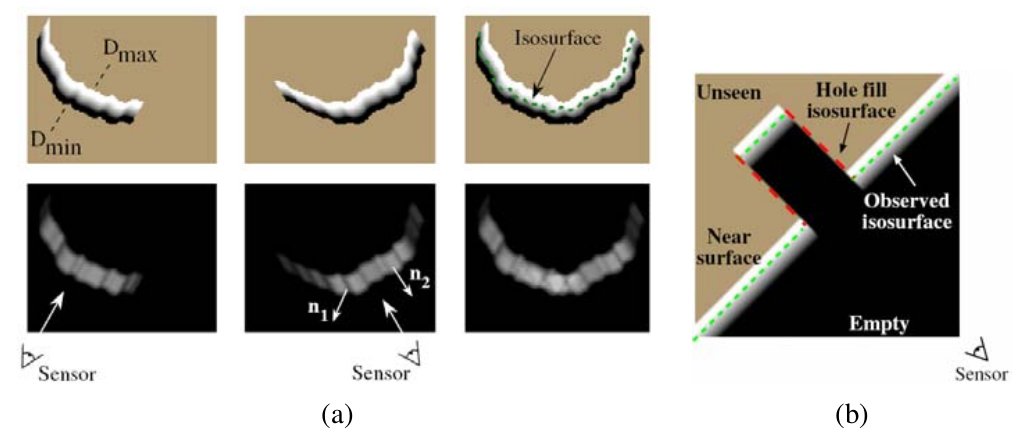
\includegraphics[width=0.8\textwidth]{fusaoDeDadosDeIntervalo.png}
    \caption{Fusão de dados de faixa (Curless e Levoy 1996) c ACM: (a) duas funções de distância assinadas (parte superior esquerda) são mescladas com seu (pesos) parte inferior esquerda para produzir um conjunto combinado de funções (coluna direita) a partir das quais uma isosuperfície pode ser extraído (linha tracejada verde); (b) as funções de distância assinadas são combinadas com rótulos de espaços vazios e não vistos para preencher buracos na superfície iso-superficial.}
    \label{fig:fusaoDeDadosDeIntervalo}
\end{figure}

A Figura \ref{fig:fusaoDeDadosDeIntervalo} mostra uma dessas abordagens, a técnica de processamento de imagens por faixa volumétrica (VRIP) desenvolvida por Curless e Levoy (1996), que primeiro calcula uma função de distância com sinal de peso de cada imagem de intervalo e as mescla usando um processo de média ponderada. Para tornar a representação mais compacta, a codificação de comprimento de execução é usada para codificar os voxels vazios, vistos e variáveis (distância sinalizada), e somente os valores de distância assinados próximos a cada superfície são armazenados.Uma vez que a função de distância assinada mesclada foi computada, um algoritmo de extração de superfície de cruzamento zero, como \textit{marching cubes} (Lorensen e Cline 1987), pode ser usado para recuperar um modelo de superfície em malha.

Técnicas de fusão de dados de faixa volumétrica baseadas em distância sinalizada ou funções características (dentro e fora) também são amplamente usadas para extrair superfícies lisas e bem comportadas de conjuntos de pontos orientados ou não orientados (Hoppe, DeRose, Duchamp et al. 1992; Ohtake, Belyaev, Alexa et al., 2003; Kazhdan, Bolitho e Hoppe, 2006; Lempitsky e Boykov, 2007; Zach, Pock e Bischof, 2007b; Zach, 2008).

\subsection{Aplicação: Herança digital}
\label{subSec:digitalHeritage}

As tecnologias ativas de identificação de alcance, combinadas com modelagem de superfície e técnicas de modelagem de aparência, são amplamente utilizadas nos campos de preservação arqueológica e histórica, que frequentemente também é denominada patrimônio digital (MacDonald 2006). Em tais aplicações, modelos 3D detalhados de objetos culturais são adquiridos e posteriormente usados para aplicações como análise, preservação, restauração e produção de obras de arte duplicadas (Rioux e Bird, 1993).

Um exemplo mais recente de tal empreendimento é o projeto Digital Michelangelo de Levoy, Pulli, Curless et al. (2000), que usaram escaneamento de tarja a laser \textit{Cyberware} e câmeras digitais SLR de alta qualidade montadas em um grande pórtico para obter digitalizações detalhadas do David de Michelangelo e outras esculturas em Florença. O projeto também fez varreduras da \textit{Forma Urbis Romae}, um antigo mapa de pedra de Roma que se despedaçou, para o qual novas características foram obtidas usando técnicas digitais. Todo o processo, desde o planejamento inicial até o desenvolvimento, aquisição e pós-processamento de \textit{software}, levou vários anos (e muitos voluntários) e, como resultado, produziu uma riqueza de técnicas de modelagem de formas e aparências em 3D.

Projetos de escala ainda maior estão sendo tentados, por exemplo, a varredura de locais completos do templo, como Angkor-Thom (Ikeuchi e Sato 2001; Ikeuchi e Miyazaki 2007; Banno, Masuda, Oishi et al. 2008).



\section{Representação de superfícies}

Nesta seção vamos analisar as representações com mais detalhe. Representações explícitas de superfície, como malhas triangulares, \textit{splines} (Farin 1992, 1996) e superfícies de subdivisão (Stollnitz, DeRose, and Salesin 1996; Zorin, Schröder, and Sweldens 1996; Warren and Weimer 2001; Peters and Reif 2008), permitindo não apenas a criação de modelos altamento detalhados, mas também operações de processamento, como a interpolação (Seção \ref{subsec:InterpolacaoDeSuperficie}), carenagem ou suavização, dizimação e simplificação (Seção \ref{subsec:SimplificacaoDeSuperficie}).

\subsection{Interpolação de superfície}
\label{subsec:InterpolacaoDeSuperficie}

Uma das operações mais comuns em superfícies é a sua reconstrução a partir de um conjunto de restrições de dados esparsos, ou seja, interpolação de dados dispersos. Ao formular tais problemas, as superfícies podem ser parametrizadas como campos de altura $\[f(\textbf{x})\]$, como superfícies paramétricas 3D $\[\textbf{f}(\textbf{x})\]$, ou como modelos não paramétricos, como coleções de triângulos.

Sabemos que os problemas de interpolação de função bidimensional e de aproximação $\[d_i \rightarrow f(x)\]$ poderiam ser lançados como problemas de minimização de energia usando a regularização. Tais problemas também podem especificar os locais de descontinuidades na superfície, bem como as restrições de orientação local (Terzopoulos 1986b; Zhang, Dugas-Phocion, Samson et al. 2002).

Uma abordagem para resolver esses problemas é a discretização da superfície e da energia em uma malha ou malha discreta usando análise de elementos finitos (Terzopoulos, 1986b). Tais problemas podem então ser resolvidos usando técnicas esparsas de solução de sistemas, como o multigrid (Briggs, Henson e McCormick 2000) ou gradiente de conjugado hierarquicamente pré-condicionado (Szeliski 2006b). A superfície também pode ser representada usando uma combinação hierárquica de B-splines multiníveis (Lee, Wolberg e Shin 1996).

Uma abordagem alternativa é usar funções de base radial (\textit{kernel}) (Boult e Kender, 1986; Nielson, 1993) para interpolar um campo $\[f(x)\]$ até um número de valores de dados $\[d_i\]$ localizado em $\[x_i\]$, a abordagem da função de base radial usa a fórmula presenta na Figura \ref{fig:baseRadial}. Onde os pesos (Figura \ref{fig:calduloPeso}), são calculados usando uma função de base radial (esférica simétrica) K(r).

\begin{figure}[!htb]
    \centering
    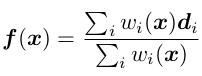
\includegraphics[width=0.3\textwidth]{radialBasisFunction.jpg}
    \caption{Função de base radial (Boult e Kender, 1986; Nielson, 1993)}
    \label{fig:baseRadial}
\end{figure}

\begin{figure}[!htb]
    \centering
    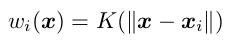
\includegraphics[width=0.4\textwidth]{weightCalcule.jpg}
    \caption{Calculo do peso}
    \label{fig:calduloPeso}
\end{figure}

Se quisermos que a função $\[f(x)\]$ interpole exatamente os pontos de dados, as funções do kernel devem ser singulares na origem, $\lim_{r\to0}$ $K(r)\rightarrow\infty$(Nielson 1993), ou um sistema linear denso deve ser resolvido para determinar a magnitude associada a cada função de base (Boult e Kender 1986). Acontece que, para certos problemas regularizados, existem funções de base radial (\textit{kernels}) que dão os mesmos resultados que uma solução analítica completa (Boult e Kender 1986). Infelizmente, porque a solução densa do sistema é cúbica no número de pontos de dados, abordagens de função de base só podem ser usadas para pequenos problemas (Beier e Neely, 1992).

Quando uma superfície paramétrica tridimensional está sendo modelada, a função com valor de vetor $\[\textbf{f}\]$ (Figura \ref{fig:baseRadial}) codifica as coordenadas 3D \textit{(x, y, z)} na superfície e o domínio x = \textit{(s, t)} codifica a parametrização da superfície. Um exemplo destas superfícies são modelos paramétricos em busca de simetria, que são versões deformáveis elasticamente de cilindros generalizados (Terzopoulos, Witkin e Kass, 1987). Nestes modelos, \textit{s} é o parâmetro ao longo da espinha do tubo deformável e \textit{t} é o parâmetro em torno do tubo. Uma variedade de suavidade e forças de simetria radial são usadas para restringir o modelo enquanto ele é ajustado para curvas de silhueta baseadas em imagem.

Também é possível definir modelos de superfícies não paramétricas, como malhas trianguladas gerais, e equipar tais malhas com métricas internas de suavidade e métricas de ajuste de dados externos (Sander e Zucker, 1990; Fua e Sander, 1992; Delingette, Hebert e Ikeuichi 1992; McInerney e Terzopoulos 1993). Enquanto a maioria dessas abordagens assume um modelo padrão de deformação elástica, que usa termos de suavidade interna quadrática, também é possível usar modelos de energia sub-linear para preservar melhor os vincos superficiais (Diebel, Thrun e Brünig 2006). As malhas triangulares também podem ser aumentadas com elementos \textit{spline} (Sullivan e Ponce, 1998) ou superfícies subdivididas (Stollnitz, DeRose e Salesin, 1996; Zorin, Schröder e Sweldens, 1996; Warren e Weimer, 2001; Peters e Reif, 2008) para produzir superfícies com melhor controle de suavidade.

Os modelos de superfície paramétricos e não paramétricos assumem que a topologia da superfície é conhecida e fixada antecipadamente. Para modelagem de superfície mais flexível, podemos representar a superfície como uma coleção de pontos orientados ou usar funções implícitas 3D, que também podem ser combinadas com modelos de superfície 3D elásticos (McInerney e Terzopoulos 1993).

\subsection{Simplificação de superfície}
\label{subsec:SimplificacaoDeSuperficie}

Uma vez que uma malha triangular tenha sido criada a partir de dados 3D, muitas vezes é desejável criar uma hierarquia de modelos de malha, por exemplo, para controlar o nível de detalhe (\textit{level of detail}) exibido em um aplicativo de computação gráfica.

Uma maneira para se fazer isso é aproximar uma dada malha com uma que tenha conectividade de subdivisão, sobre a qual um conjunto de coeficientes triangulares \textit{wavelet} pode então ser computado (Eck, DeRose, Duchamp et al. 1995). Uma abordagem mais contínua é usar operações sequenciais de colapso de borda para ir da malha de resolução fina original para uma malha de nível básico grosseira (Hoppe 1996).

\begin{figure}[!htb]
    \centering
    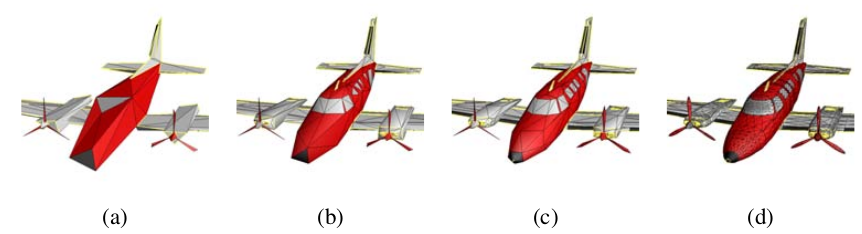
\includegraphics[width=0.7\textwidth]{malhaProgressiva.png}
    \caption{Representação de malha progressiva de um modelo de avião (Hoppe 1996)}
    \label{fig:malhaProgressiva}
\end{figure}

A representação resultante da malha progressiva pode ser usada para renderizar o modelo 3D em níveis arbitrários de detalhe, como mostrado na Figura \ref{fig:malhaProgressiva}.

Na Figura \ref{fig:malhaProgressiva}a foi utilizado uma malha de base $\[\textit{M}^{0}\]$ (total de 150 faces), na sequência (\ref{fig:malhaProgressiva}b) a malha de base foi de $\[\textit{M}^{175}\]$ (totalizando 500 faces), a terceira (\ref{fig:malhaProgressiva}c) malha de base foi de $\[\textit{M}^{425}\]$ (1000 faces) e por último (\ref{fig:malhaProgressiva}d) uma malha de base original $\[\textit{M = M}^n\]$, sendo esta totalizando 13,546 faces.

\subsection{Imagens de geometria}

Enquanto representações de superfície de multi-resolução suportam operações de nível de detalhes, elas ainda consistem em uma coleção irregular de triângulos, o que dificulta comprimir e armazenar em cache de maneira eficiente.

Para tornar a triangulação completamente regular (uniforme e quadriculado), Gu, Gortler e Hoppe (2002) descrevem como criar imagens geométricas cortando malhas de superfície ao longo de linhas bem escolhidas e “achatando” a representação resultante em um quadrado.

\begin{figure}[!htb]
    \centering
    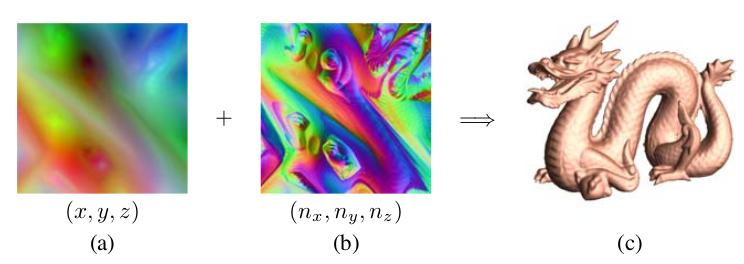
\includegraphics[width=0.7\textwidth]{imagemDeGeometria.jpg}
    \caption{Imagens de geometria (Gu, Gortler e Hoppe 2002) ACM: (a) 257x257 imagem de geometria define uma malha sobre a superfície; (b) mapa normal de 512x512 que define o vértice normal; (c) modelo 3D final iluminado.}
    \label{fig:imagemGeometria}
\end{figure}

A Figura \ref{fig:imagemGeometria}a mostra os valores resultantes \textit{(x, y, z)} da malha de superfície mapeada sobre o quadrado unitário, enquanto a Figura \ref{fig:imagemGeometria}b mostra o mapa normal associado \textit{(nx, ny, nz)}, ou seja, as normais de superfície associadas a cada malha vértice, que pode ser usado para compensar a perda de fidelidade visual se a imagem da geometria original estiver muito comprimida.

\section{Reconstrução baseada em modelos}
Quando sabemos algo antecipadamente sobre os objetos que estamos tentando modelar, podemos construir modelos 3D mais detalhados e confiáveis usando técnicas e representações especializadas. Por exemplo, a arquitetura é geralmente composta de grandes regiões planares e outras formas paramétricas (como superfícies de revolução), geralmente perpendiculares à gravidade e entre si (Seção \ref{subsec:Arquitetural}). Cabeças e faces podem ser representados usando modelos de formato não-rígido, de baixa dimensionalidade, uma vez que a variabilidade na forma e na aparência de faces humanas, embora extremamente grande, ainda é limitada (Seção 12.6.2). Os corpos humanos ou partes, como as mãos, formam estruturas altamente articuladas, que podem ser representadas usando cadeias cinemáticas de elementos esqueletais rígidos por partes ligados por articulações (Seção 12.6.4).

Nesta seção, destacamos algumas das principais ideias, representações e algoritmos de modelagem usados para esses três casos. Detalhes e referências adicionais podem ser encontrados em conferências especializadas e workshops dedicados a esses tópicos, por exemplo, o Simpósio Internacional de Processamento 3D de Dados, Visualização e Transmissão (3DPVT), a Conferência Internacional sobre Modelação e Imagens Digitais 3D (3DIM), a Conferência Internacional sobre Rosto Automático e Reconhecimento de Gestos (FG), o Workshop IEEE sobre Análise e Modelagem de Rostos e Gestos, e o Workshop Internacional sobre Rastreamento de Seres Humanos para a Avaliação de seus Movimentos em Seqüências de Imagens (THEMIS).

\subsection{Arquitetural}
\label{subsec:Arquitetural}
O trabalho de Debevec, Taylor e Malik (1996)\cite{Debevec:1996:MRA:237170.237191} foi um dos primeiros sistemas de modelagem e renderização híbridos baseados em geometria e imagem. Seu sistema chamado Façade combina uma ferramenta de modelagem geométrica interativa guiada por imagem com correspondência estereofônica baseada em modelo e mapeamento de textura dependente da visão. Durante a fase de modelagem fotogramétrica interativa, o usuário seleciona elementos de bloco e alinha suas bordas com bordas visíveis nas imagens de entrada (Figura \ref{fig:img1}a). O sistema calcula automaticamente as dimensões e localizações dos blocos junto com as posições da câmera usando otimização restrita.

\begin{figure}[!htb]
    \centering
    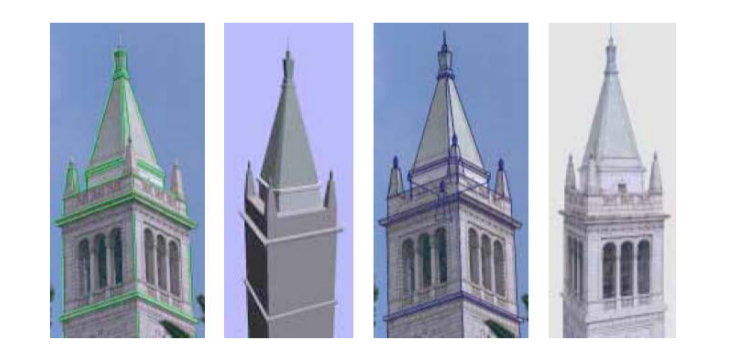
\includegraphics[width=0.7\textwidth]{img1.png}
    \caption{Modelagem arquitetural interativa usando o sistema Façade (Debevec, Taylor e Malik 1996) c 1996 ACM: (a) imagem de entrada com bordas desenhadas pelo usuário mostradas em verde; (b) modelo sólido 3D sombreado; (c) primitivas geométricas sobrepostas à imagem de entrada; (d) modelo 3D final, dependente de visão e mapeado por textura.}
    \label{fig:img1}
\end{figure}

(Figura \ref{fig:img1}b-c). Essa abordagem é intrinsecamente mais confiável do que a estrutura geral baseada em recursos do movimento, porque explora a geometria forte disponível nas primitivas de bloco. Trabalhos relacionados de Becker e Bove (1995)\cite{Becker}, Horry, Anjyo e Arai (1997)\cite{Horry:1997:TPU:258734.258854} e Criminisi, Reid e Zisserman (2000)\cite{Criminisi00a} exploram informações similares disponíveis a partir de pontos de fuga. No sistema interativo de modelagem baseada em imagens de Sinha, Steedly, Szeliski et al. (2008)\cite{Sinha:2008:IAM:1409060.1409112}, as direções dos pontos de fuga são usadas para guiar o usuário no desenho de polígonos, que são então automaticamente encaixados em pontos 3D esparsos recuperados usando a estrutura do movimento.

Uma vez que a geometria aproximada foi estimada, mapas de deslocamento mais detalhados podem ser calculados para cada face plana usando uma varredura de plano local, que Debevec, Taylor e Malik (1996)\cite{Debevec:1996:MRA:237170.237191} chamam de estéreo baseado em modelo. Finalmente, durante a renderização, as imagens de diferentes pontos de vista são distorcidas e misturadas à medida que a câmera se move pela cena, usando um processo chamado mapeamento de textura dependente da visão (Figura \ref{fig:img1}d).

Para modelagem de interiores, em vez de trabalhar com imagens individuais, é mais útil trabalhar com panoramas, já que você pode ver extensões maiores de paredes e outras estruturas. O sistema de modelagem 3D desenvolvido por Shum, Han e Szeliski (1998)\cite{Shum1998InteractiveCO} primeiro constrói panoramas calibrados a partir de múltiplas imagens e então faz o usuário desenhar linhas verticais e horizontais na imagem para demarcar os limites das regiões planas. As linhas são inicialmente usadas para estabelecer uma rotação absoluta para cada panorama e são usadas posteriormente (juntamente com os vértices e planos inferidos) para otimizar a estrutura 3D, que pode ser recuperada até a escala de uma ou mais imagens (Figura \ref{fig:img2}). Os panoramas de alta faixa dinâmica de 360º também podem ser usados para modelagem externa, pois fornecem estimativas altamente confiáveis de orientações relativas de câmera, bem como direções de pontos de fuga (Antone e Teller, 2002)\cite{Antone:2002:SEC:598434.598520}.

\begin{figure}[!htb]
    \centering
    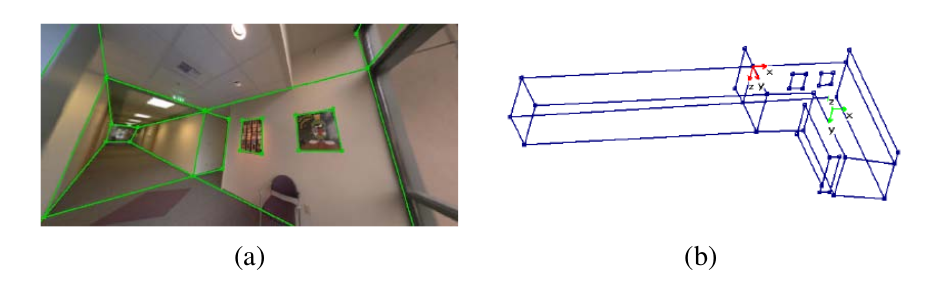
\includegraphics[width=0.7\textwidth]{img2.png}
    \caption{Modelagem 3D interativa a partir de panoramas (Shum, Han e Szeliski, 1998)\cite{Shum1998InteractiveCO}: (a) visão grande angular de um panorama com linhas verticais e horizontais (alinhadas ao eixo) desenhadas pelo usuário; (b) reconstrução de vista única dos corredores.}
    \label{fig:img2}
\end{figure}

Enquanto os sistemas de modelagem baseados em imagem anteriores exigiam alguma autoria do usuário, Werner e Zisserman (2002)\cite{Werner} apresentam um sistema de reconstrução baseado em linhas totalmente automatizadas. Eles primeiro detectam linhas e pontos de fuga e os usam para calibrar a câmera; em seguida, eles estabelecem correspondências de linha usando os dois tensores de correspondência de aparência e trifocais, o que permite reconstruir famílias de segmentos de linha 3D, como mostrado na Figura \ref{fig:img3}a. Eles então geram hipóteses planas, usando linhas 3D coplanares e uma varredura de plano com base nos escores de correlação cruzada avaliados em pontos de interesse. Interseções de planos são usadas para determinar a extensão de cada plano, ou seja, uma geometria grosseira inicial, que é então refinada com a adição de recortes e extrusões retangulares ou em forma de cunha (Figura \ref{fig:img3}c).

\begin{figure}[!htb]
    \centering
    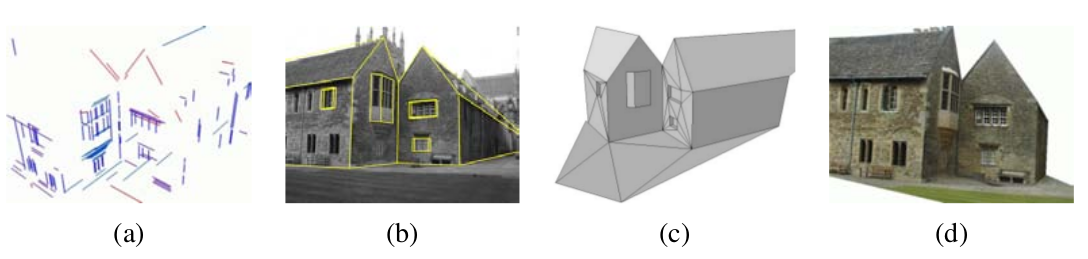
\includegraphics[width=0.7\textwidth]{img3.png}
    \caption{Reconstrução arquitetônica automatizada usando linhas e planos 3D (Werner e Zisserman 2002)\cite{Werner}: (a) linhas 3D reconstruídas, codificadas por cores por suas direções de fuga; (b) modelo de armação de arame sobreposto a uma imagem de entrada; (c) modelo triangular triangular com janelas; (d) modo final de mapeamento de textura
}
    \label{fig:img3}
\end{figure}

\subsection{Cabeças e rostos}
Outra área em que modelos especializados de forma e aparência são extremamente úteis é na modelagem de cabeças e faces. Embora a aparência das pessoas pareça infinitamente variável à primeira vista, a forma real da cabeça e da face de uma pessoa pode ser descrita razoavelmente bem usando algumas dezenas de parâmetros.

A Figura \ref{fig:img4} mostra um exemplo de um sistema de modelagem baseado em imagem, em que os pontos-chave especificados pelo usuário em várias imagens são usados para ajustar um modelo de cabeçalho genérico ao rosto de uma pessoa. Como você pode ver na Figura \ref{fig:img4}c, depois de especificar apenas mais de 100 pontos chave, a forma da face se tornou bastante adaptada e reconhecível. Extrair um mapa de textura das imagens originais e, em seguida, aplicá-lo ao modelo de cabeçote resulta em um modelo animado com notável fidelidade visual (Figura \ref{fig:img5}a).


\begin{figure}[!htb]
    \centering
    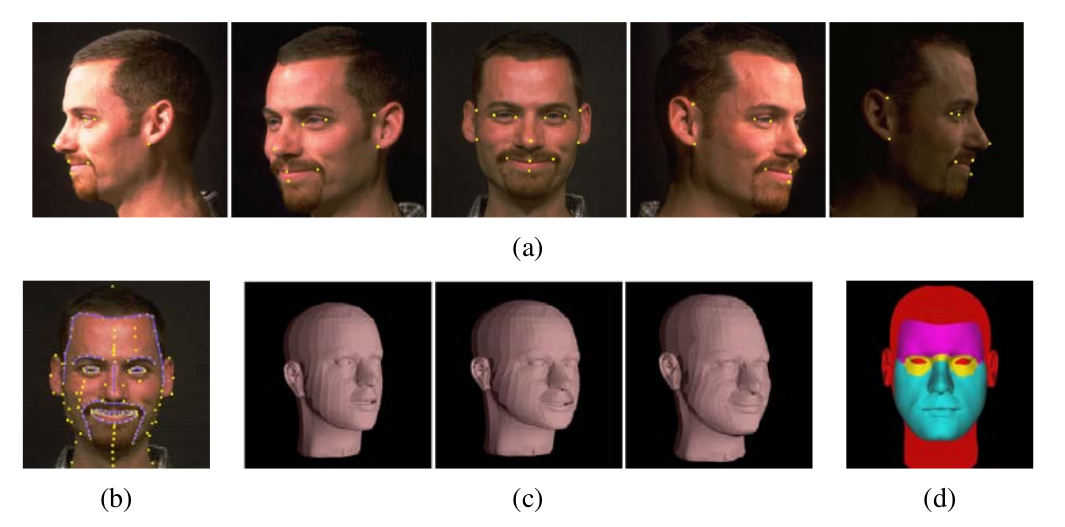
\includegraphics[width=0.7\textwidth]{img4.png}
    \caption{Adaptação do modelo 3D a uma coleção de imagens: (Pighin, Hecker, Lischinski et al. 1998): (a) conjunto de cinco imagens de entrada junto com pontos chave selecionados pelo usuário; (b) o conjunto completo de pontos chave e curvas; (c) três malhas - o original, adaptado após 13 pontos chave, e após 99 pontos chave adicionais; (d) a partição da imagem em regiões animadas separadamente.
}
    \label{fig:img4}
\end{figure}

\begin{figure}[!htb]
    \centering
    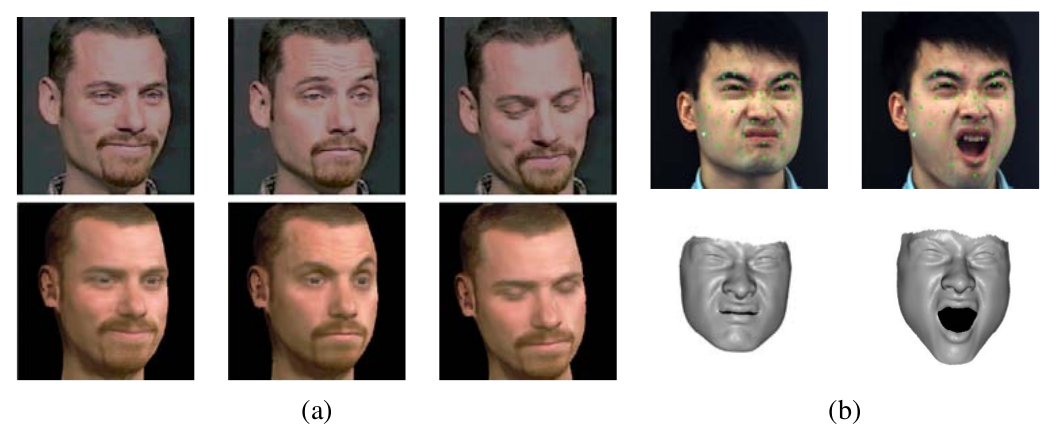
\includegraphics[width=0.7\textwidth]{img5.png}
    \caption{Rastreamento e reanimação de cabeças e expressões usando modelos 3D deformáveis. (a) Os modelos se ajustam diretamente a cinco fluxos de vídeo de entrada (Pighin, Szeliski e Salesin 2002): A linha inferior mostra os resultados da nova animação de um modelo 3D sintético mapeado por textura com parâmetros de pose e expressão ajustados às imagens de entrada fileira superior. (b) Modelos ajustados a modelos de superfícies estéreo de frame-rate estéreo (Zhang, Snavely, Curless et al. 2004): A linha superior mostra as imagens de entrada com marcadores verdes sintéticos sobrepostos, enquanto a linha inferior mostra a superfície 3D ajustada modelo.
}
    \label{fig:img5}
\end{figure}

Um sistema mais poderoso pode ser construído aplicando-se a análise de componentes principais (PCA) a uma coleção de faces digitalizadas em 3D. Como você pode ver na Figura \ref{fig:img6}, é possível, então, ajustar modelos 3D mais simples a imagens individuais e usar tais modelos para uma variedade de efeitos visuais e de animação (Blanz e Vetter, 1999)\cite{Blanz:1999:MMS:311535.311556}.

\begin{figure}[!htb]
    \centering
    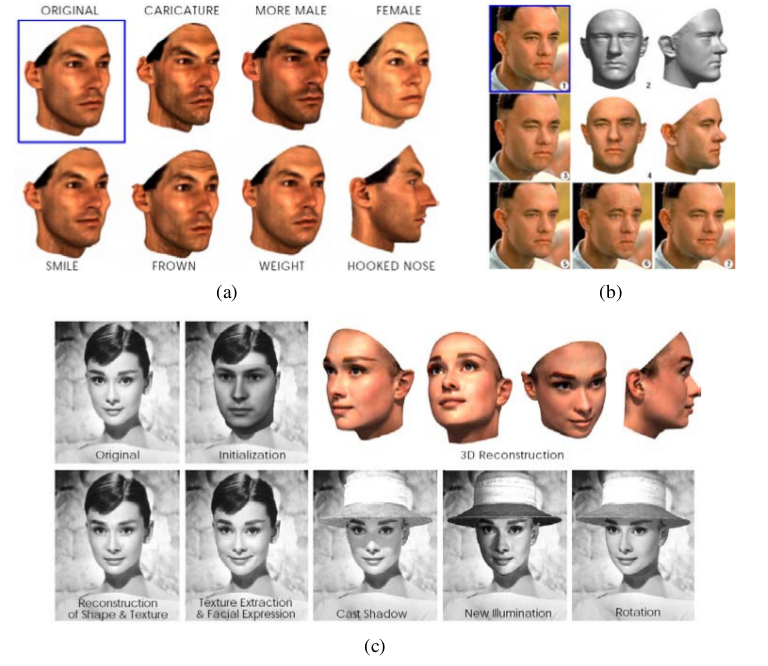
\includegraphics[width=0.7\textwidth]{img6.png}
    \caption{Modelo 3D de faces morfáveis (Blanz e Vetter 1999)\cite{Blanz:1999:MMS:311535.311556}: (a) modelo 3D original com adição de variações de forma e textura em direções específicas: desvio da média (caricatura), gênero, expressão, peso e formato do nariz ; (b) um modelo 3D morfável é ajustado a uma única imagem, após a qual seu peso ou expressão pode ser manipulado; (c) outro exemplo de uma reconstrução 3D, juntamente com um conjunto diferente de manipulações 3D, como iluminação e mudança de pose.
}
    \label{fig:img6}
\end{figure}

\subsection{Aplicação: Animação Facial}
Talvez a aplicação mais amplamente utilizada na modelagem de cabeças 3D seja a animação facial. Uma vez que um modelo 3D parametrizado de forma e aparência (textura da superfície) tenha sido construído, ele pode ser usado diretamente para rastrear os movimentos faciais de uma pessoa (Figura \ref{fig:img5}a) e para animar um personagem diferente com esses mesmos movimentos e expressões.

\subsection{Modelagem e rastreamento de corpo inteiro}
Os tópicos de rastreamento de seres humanos, modelagem de sua forma e aparência e reconhecimento de suas atividades, são algumas das áreas mais ativamente estudadas da visão computacional. Neste Seção levantaremos alguns tópicos importantes na detecção e rastreamento de seres humanos.

\subsubsection{Subtração de fundo}
Um dos primeiros passos em muitos é modelar o fundo para extrair os objetos em movimento correspondentes às pessoas. Toyama, Krumm, Brumitt et al. (1999) revisam várias técnicas de manutenção de fundo de fosqueamento de diferenças e fornecem uma boa introdução a este tópico. Sidenbladh e Black (2003) desenvolvem um tratamento mais abrangente, que modela não apenas as estatísticas da imagem de fundo, mas também a aparência dos objetos em primeiro plano, estatísticas (diferença de quadros). Uma vez que as silhuetas tenham sido extraídas de uma ou mais câmeras, elas podem ser modeladas usando modelos deformáveis ou outros modelos de contorno (Baumberg e Hogg 1996; Wren, Azarbayejani, Darrell et al. 1997).

\subsubsection{Inicialização e detecção}
Para rastrear pessoas de maneira totalmente automatizada, é necessário primeiro detectar sua presença em quadros de vídeo individuais. Este tópico está intimamente relacionado à detecção de pedestres, que é frequentemente considerada como um tipo de reconhecimento de objetos (Mori, Ren, Efros et al. 2004; Felzenszwalb e Huttenlocher 2005; Felzenszwalb, McAllester e Ramanan 2008). Técnicas adicionais para inicializar rastreadores 3D baseados em imagens 2D incluem aquelas descritas por Howe, Leventon e Freeman (2000), Rosales e Sclaroff (2000), Shakhnarovich, Viola e Darrell (2003), Sminchisescu, Kanaujia, Li et al. (2005), Agarwal e Triggs (2006), Lee e Cohen (2006), Sigal e Black (2006), e Stenger, Thayananthan, Torr et al. (2006). Técnicas de rastreamento quadro a quadro pode ser utilizadas para fornecer melhor confiabilidade na detecção (Fossati, Dimitrijevic, Lepetit et al. 2007; Andriluka, Roth e Schiele 2008; Ferrari, Marin-Jimenez e Zisserman 2008).

\subsubsection{Acompanhamento com fluxo}
O rastreamento de pessoas e sua postura de um quadro para outro podem ser aprimorados pela computação do fluxo óptico ou pela correspondência da aparência de seus membros de um quadro para outro. Por exemplo, o modelo de pessoas de papelão de Ju, Black e Yacoob (1996) modela a aparência de cada porção de perna (superior e inferior) como um retângulo móvel e usa fluxo óptico para estimar sua localização em cada quadro subseqüente. Cham e Rehg (1999) e Sidenbladh, Black e Fleet (2000) rastreiam membros usando fluxo óptico e templates, juntamente com técnicas para lidar com múltiplas hipóteses e incertezas. Bregler, Malik e Pullen (2004) usam um modelo 3D completo do movimento dos membros e do corpo, como descrito abaixo.

\subsubsection{Modelos cinemáticos 3D}
A eficácia da modelagem e do rastreamento humano pode ser bastante aprimorada usando um modelo 3D mais preciso da forma e do movimento de uma pessoa. Subjacente a tais representações, que são onipresentes na animação 3D em jogos e efeitos especiais, está um modelo cinemático ou cadeia cinemática, que especifica o comprimento de cada membro em um esqueleto, bem como os ângulos de rotação 2D ou 3D entre os membros ou segmentos ( Figura \ref{fig:img7}a-b).
A Figura \ref{fig:img7}a mostra o modelo cinemático de uma mão humana usada por Rehg, Morris e Kanade (2003) para rastrear o movimento da mão em um vídeo. Como você pode ver, os pontos de ligação entre os dedos e os polegares têm dois graus de liberdade, enquanto as articulações dos dedos têm apenas um. O uso desse tipo de modelo pode aumentar consideravelmente a capacidade de um rastreador baseado em borda para lidar com movimento rápido, ambigüidades em pose 3D e oclusões parciais. Os modelos de cadeia cinemática são ainda mais amplamente utilizados para modelagem e rastreamento de todo o corpo (O'Rourke e Badler, 1980; Hogg, 1983; Rohr, 1994). Observe que algumas técnicas usam modelos 2D acoplados a medições 2D, alguns usam medições 3D (dados de intervalo ou vídeo com várias visualizações) com modelos 3D e alguns usam vídeo monocular para inferir e rastrear modelos 3D diretamente. Também é possível usar modelos temporais para melhorar o rastreamento de movimentos periódicos, como caminhar, analisando os ângulos articulares como funções do tempo (Polana e Nelson, 1997; Seitz e Dyer, 1997; Cutler e Davis, 2000). A generalidade e a aplicabilidade de tais técnicas podem ser melhoradas aprendendo padrões típicos de movimento usando a análise de componentes principais (Sidenbladh, Black e Fleet 2000; Urtasun, Fleet e Fua 2006).

\begin{figure}[!htb]
    \centering
    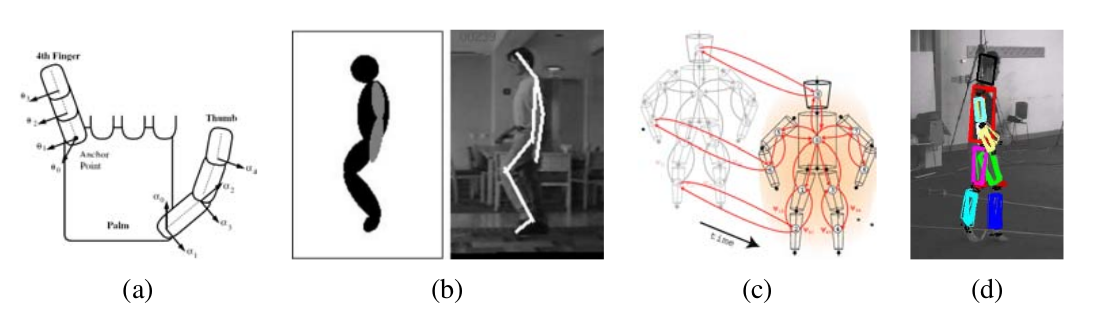
\includegraphics[width=0.7\textwidth]{img8.png}
    \caption{Rastreamento do movimento humano em 3D: (a) modelo de cadeia cinemática para uma mão humana (Rehg, Morris e Kanade 2003), reimpresso com permissão da SAGE; (b) seguir um modelo de blob de cadeia cinemática numa sequência de vídeo (Bregler, Malik e Pullen 2004); (c-d) coleção probabilística de membros soltos de partes do corpo (Sigal, Bhatia, Roth et al. 2004)
}
    \label{fig:img7}
\end{figure}

\subsubsection{Modelos probabilísticos}
Como o rastreamento pode ser uma tarefa tão difícil, técnicas sofisticadas de inferência probabilística são frequentemente usadas para estimar os prováveis estados das pessoas que estão sendo rastreadas. Uma abordagem popular, chamada filtragem de partículas (Isard e Blake, 1998), foi originalmente desenvolvida para rastrear os contornos de pessoas e mãos. Subsequentemente, ele foi aplicado ao rastreamento de todo o corpo (Deutscher, Blake e Reid, 2000; Sidenbladh, Black e Fleet, 2000; Deutscher e Reid, 2005) e continua a ser usado em rastreadores modernos (Ong, Micilotta, Bowden et al. 2006). Abordagens alternativas para lidar com a incerteza inerente ao rastreamento incluem o rastreamento de múltiplas hipóteses (Cham e Rehg, 1999) e covariâncias infladas (Sminchisescu e Triggs, 2001). A Figura \ref{fig:img7}c-d mostra um exemplo de um sofisticado modelo gráfico probabilístico espaço-temporal, que modela não apenas a relação geométrica entre vários membros, mas também sua provável dinâmica temporal (Sigal, Bhatia, Roth et al. 2004 ).

\subsubsection{Modelagem de forma adaptativa}
Outro componente essencial da modelagem e rastreamento de todo o corpo é a adaptação de modelos de forma parametrizados a dados visuais. Os conjuntos de dados registados são utilizados para modelar a variação na forma como uma função das características pessoais e da pose do esqueleto, por exemplo, o abaulamento dos músculos, como certas articulações são flexionadas (Figura \ref{fig:img8}). O sistema resultante pode então ser utilizado para a conclusão da forma, isto é, a recuperação de um modelo de malha 3D completo a partir de um pequeno número de marcadores capturados, encontrando os melhores parâmetros de modelo tanto no formato como no espaço de posicionamento que se ajustam aos dados medidos. Enquanto os sistemas de estimativa de encaixe e pose de corpo anteriores usam múltiplas vistas para estimar a forma do corpo, um trabalho ainda mais recente de Guan, Weiss, Bǎlan et al. (2009) pode encaixar uma forma humana e representar o modelo para uma única imagem de uma pessoa em um fundo natural. A inicialização manual é usada para estimar um modelo de pose áspera (esqueleto) e altura, e isso é usado para segmentar o contorno da pessoa usando o algoritmo de segmentação Grab Cut. A estimativa da forma e da pose é então refinada usando uma combinação de dicas de borda de silhueta e informações de sombreamento (Figura \ref{fig:img8}). O modelo 3D resultante pode ser usado para criar novas animações.


\begin{figure}[!htb]
    \centering
    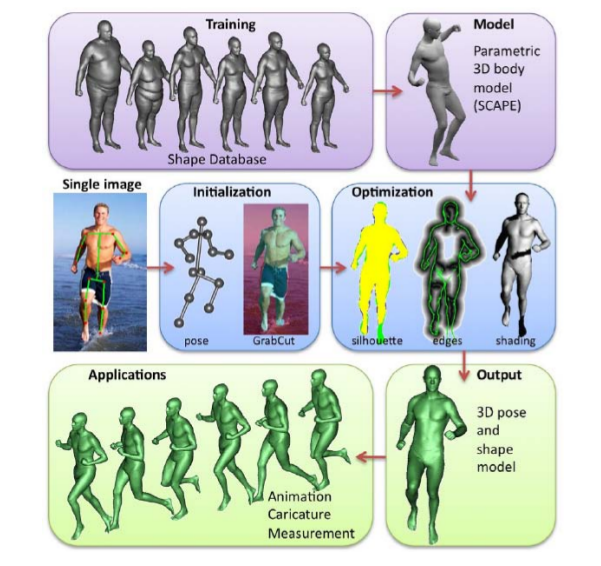
\includegraphics[width=0.7\textwidth]{img7.png}
    \caption{Estimando a forma humana e pose de uma única imagem usando um modelo 3D paramétrico (Guan, Weiss, Bǎlan et al. 2009).
}
    \label{fig:img8}
\end{figure}


\subsubsection{Reconhecimento de atividade}
O tema final amplamente estudado na modelagem humana é o reconhecimento de movimento, atividade e ação (Bobick, 1997; Hu, Tan, Wang e outros, 2004; Hilton, Fua e Ronfard, 2006). Exemplos de ações que são comumente reconhecidas incluem andar e correr, pular, dançar, pegar objetos, sentar e levantar e acenar. Trabalhos representativos recentes sobre esses tópicos foram escritos por Robertson e Reid (2006), Sminchisescu, Kanaujia e Metaxas (2006), Weinland, Ronfard e Boyer (2006), Yilmaz e Shah (2006) e Gorelick, Blank, Shechtman. et al. (2007).


% References
\clearpage
\small
\bibliographystyle{plain}
\bibliography{bibliography}

\end{document}



